\documentclass[12pt, letterpaper]{article}
\usepackage[utf8]{inputenc}

\usepackage{amsthm}
\usepackage{amssymb}
\usepackage{amsmath}
\usepackage{mathtools}
\usepackage{amsfonts}
\usepackage{graphicx}
\usepackage{algpseudocode}
\usepackage{algorithm}
\usepackage{tikz}
\usepackage{paralist}
\usepackage{listings}
\usepackage{bookmark}
\usepackage{physics}
\usepackage{cancel}
\input{insbox}
\usepackage{titling}
\usepackage{xcolor}
\usepackage{circuitikz}


\renewcommand\maketitlehooka{\null\mbox{}\vfill}
\renewcommand\maketitlehookd{\vfill\null}

\usetikzlibrary{arrows, automata}

\graphicspath{ {./images/} }

\makeatletter
\pdfstringdefDisableCommands{\let\HyPsd@CatcodeWarning\@gobble}
\makeatother

\title{
  \Large $\textbf{Radio Frequency Circuits \& Antenna}$
}
\author{
  $\textbf{Thomas Glezer}$\\
  $\textbf{Tel Aviv University}$\\\\
  ---\\\\
  $\textbf{Homework: 5}$\\
}
\date{\today}



\begin{document}

\begin{titlingpage}
  \maketitle
\end{titlingpage}

\pagebreak

\section{Complete the entries in the following table:}

\vspace{2em}
Remarks on general equations:
\vspace{2em}

\begin{align}
  VSWR
  &=
  {1+|\Gamma|\over1-|\Gamma|}
  \Longleftrightarrow
  |\Gamma|
  =
  \Big|{1-VSWR\over1+VSWR}\Big|
  \\
  |\Gamma|&=\sqrt{P_r/P_f}
  \\
  T&=\sqrt{1-|\Gamma|^2}
  \Longleftrightarrow
  |\Gamma|=\sqrt{1-T^2}
  \\
  RL(dB) &= 10\log_{10}{P_i\over P_r} = -20\log_{10}|\Gamma|
  \Longleftrightarrow
  |\Gamma|
  =
  10^{-RL/20}
  \\
  IL(dB) &= 10\log_{10}{P_T\over P_R}
  =
  -20\log_{10}(|T|)
  \Longleftrightarrow
  |\Gamma|
  =
  \sqrt{1-10^{-IL/10}}
\end{align}

\vspace{2em}

\begin{center}
  \begin{tabular}{| c | c | c | c | c |}
    \hline
    $VSWR$ & $|\Gamma|$ & $RL(dB)$ & $|T|$ & $IL (dB)$\\
    \hline
    {\color{blue}1.02} & 0.01 & {\color{blue}40} & {\color{blue}0.99995} & {\color{blue}0.000434} \\
    \hline
    {\color{blue}1.1} & {\color{blue}0.05} & 26 & {\color{blue}0.99874} & {\color{blue}0.011} \\
    \hline
    1.22 & {\color{blue}0.099} & {\color{blue}20.078} & {\color{blue}0.995} & {\color{blue}0.04286} \\
    \hline
    {\color{blue}1.49687} & {\color{blue}0.1989997} & {\color{blue}14.023} & 0.98 & {\color{blue}0.17547} \\
    \hline
    1.86 & 0.3 & 10.5 & 0.954 & 0.41 \\
    \hline
    {\color{blue}2.337}& {\color{blue}0.40067} & {\color{blue}7.944} & {\color{blue}0.91622} & 0.76 \\
    \hline
    {\color{blue}3}& {\color{blue}0.5} & 6.02 & {\color{blue}0.866} & {\color{blue}1.249587} \\
    \hline
    4 & {\color{blue}0.6} & {\color{blue}4.437} & {\color{blue}0.8} & {\color{blue}1.9382} \\
    \hline
    {\color{blue}9} & {\color{blue}0.8} & {\color{blue}1.9365} & {\color{blue}0.6} & 4.44 \\
    \hline
  \end{tabular}
\end{center}

\pagebreak

\section{Complete the entries in the following table:}


\vspace{2em}
Remarks on general equations:

\begin{align}
  P[dBm]=10\log_{10}P[mW]\\
  P[W]=10^3P[mW]
\end{align}
\vspace{2em}

\begin{center}
  \begin{tabular}{| c | c | c |}
    \hline
    $P[W]$ & $P[mW]$ & $P[dBm]$ \\
    \hline
    $10^{-4}$ & {\color{blue}0.1} & {\color{blue}-10} \\
    \hline
    {\color{blue}$10^{-3}$} & 1 & {\color{blue}0} \\
    \hline
    {\color{blue}$10^{-2}$} & {\color{blue}10} & 10 \\
    \hline
    {\color{blue}0.015} & 15 & {\color{blue}11.76} \\
    \hline
    0.02 & {\color{blue}20} & {\color{blue}13.01} \\
    \hline
    {\color{blue}0.1} & {\color{blue}100} & 20 \\
    \hline
  \end{tabular}
\end{center}

\section{An amplifier with a gain of $11 [dB]$, a bandwidth of $150 [MHz]$, and a noise figure of $3.8 [dB]$ feeds a receiver with a noise temperature of $935 [K]$. Find the noise figure of the overall system.}

\begin{align}
  F_{tot}
  &=
  F_1
  +
  {F_2-1\over G_1}
  \\
  &=
  3.8[dB]
  +
  {1+T_e/T_o-1\over 11[dB]}
  \\
  &=
  10^{0.38}
  +
  {T_e\over10^{1.1}T_o}
  \\
  &=
  2.4
  +
  {935\over12.59\cdot290}
  =
  2.4+0.2561
  \\
  F_{tot}
  &=
  2.656
  \rightarrow
  4.242[dB]
\end{align}

\section{Consider the wireless local area network (WLAN) receiver front-end shown below, where the bandwidth of the bandpass filter is $100 [MHz]$ centered at $2.4 [GHz]$. The system is at the room temperature.}

\begin{center}
  \begin{circuitikz}
    \node [muxdemux, muxdemux def={NL=1, NR=1, NT=0, NB=0, w=6, Lh=2, Rh=2, inset Rh=1.0}](filter) at (0,0) {\parbox{1.5cm}{IL=1.5[dB]\\B=100[MHz]}};
    \draw  (filter.rpin 1) to[amp,l_={\parbox{1.5cm}{$G_2{=}10dB$\\$F_2${=}2dB}}]++(2.5,0);
    \draw  (4,0) to[amp,l_={\parbox{1.5cm}{$G_3{=}20dB$\\$F_3${=}2dB}}]++(2.5,0);
  \end{circuitikz}
\end{center}

\begin{itemize}
  \item [a)] Find the noise figure of the overall system.
  \begin{align}
    L
    =
    10^{1.5/10}=1.41
    \quad&\wedge\quad
    G_1
    =
    L^{-1}
    \\
    F_2
    =
    10^{2/10}=1.585
    \quad&\wedge\quad
    G_2
    =
    10^{10/10}
    =
    10
    \\
    F_3
    =
    10^{2/10}=1.585
    \quad&\wedge\quad
    G_3
    =
    10^{20/10}
    =
    100
  \end{align}
  \begin{align}
    F_{tot}
    &=
    F_1
    +
    {F_2-1\over G_1}
    +
    {F_3-1\over G_1G_2}
    \\
    &=
    1.41
    +
    {1.585-1\over 1/1.41}
    +
    {1.585-1\over 10/1.41}
    \\
    F_{tot}
    &=
    2.317
    \rightarrow
    3.65[dB]
  \end{align}
  \item [b)] What is the resulting signal-to-noise ratio at the output, if the input signal power level is -86 dBm?
  \begin{align}
    P_{in}
    &=
    -86[dBm]
    =
    2.512\cdot10^{-9}mW
    \\
    P_{out}
    &=
    (P_{in}+G_2+G_3-L)[dBm]
    =
    \\
    &=
    -86+10+20-1.5
    \\
    &=
    -57.5[dBm]
    \\
    &=
    1.78\cdot10^{-6}mW
  \end{align}
  Noise effect:
  \begin{align}
    N
    &=
    G\cdot K\cdot T\cdot B
    \\
    G
    &=
    -1.5+10+20
    =
    28.5[dB]
    \rightarrow
    10^{2.85}=707.95
    \\
    K&=1.38\cdot10^{-23}[J/K]
    \\
    T
    &=
    (F_{tot}-1)T_0
    =
    (2.317-1)290
    =
    381.9[K]
    \\
    B
    &=
    100[MHz]=10^8[Hz]
    \\
    \therefore
    N
    &=
    707.95\cdot
    1.38\cdot 10^{-23} \cdot
    381.9\cdot
    10^8
    \\
    &=
    3.73\cdot10^{-7}[mW]\rightarrow -64.3[dBm]
  \end{align}
  \begin{align}
    SNR
    =
    {P_{out}\over N_{out}}
    =
    -57.5-(-64.3)=6.8[dB]\rightarrow 4.79
  \end{align}
  \item [c)] Can the components be arranged to give a better noise figure?
  \\
  {\color{blue} Yes, by reversing the order of the system we would get:}
  \begin{align}
    F_{tot}
    &=
    F_1
    +
    {F_2-1\over G_1}
    +
    {F_3-1\over G_1G_2}
    \\
    &=
    1.585
    +
    {1.585-1\over 100}
    +
    {1.41-1\over 1000}
    \\
    F_{tot}
    &=
    1.59
    \rightarrow
    2.02[dB]
  \end{align}
\end{itemize}

\section{Consider the next system:}

\vspace{1em}

\begin{center}
  \begin{circuitikz}
    \node [muxdemux, muxdemux def={NL=1, NR=1, NT=0, NB=0, w=6, Lh=2, Rh=2, inset Rh=1.0}](filter) at (0,0) {Noise source};
    \draw  (filter.rpin 1) to[amp,l_={\parbox{1.5cm}{$G_1{=}23dB$\\$F_1${=}0.86dB}}]++(2.5,0);
    \node [muxdemux, muxdemux def={NL=1, NR=1, NT=0, NB=0, w=3, Lh=1, Rh=1, inset Rh=1.0}](wire) at (6,0) {};
    \draw (4, 0) to (wire.lpin 1);
    \draw  (wire.rpin 1) to[amp,l_={\parbox{1.5cm}{$G_2{=}21dB$\\$F_2${=}2.8dB}}]++(2.5,0);
  \end{circuitikz}
\end{center}

\begin{itemize}
  \item [a)] Find the equivalent noise temperature and the noise figure of the system (without the noise of the source).
  \begin{align}
    G_1
    =
    23[dB]
    \rightarrow
    199.5
    \quad&\wedge\quad
    F_1
    =
    0.86[dB]
    \rightarrow
    1.22
    \\
    L
    =
    0.9[dB]
    \rightarrow
    1.23
    \quad&\wedge\quad
    T
    =
    315
    \\
    G_2
    =
    21[dB]
    \rightarrow
    125.9
    \quad&\wedge\quad
    F_2
    =
    2.8[dB]
    \rightarrow
    1.91
  \end{align}
  \begin{align}
    T_1
    &=
    (F_1-1)T_0
    =
    (1.22-1)290=63.8[K]
    \\
    T_2
    &=
    (F_2-1)T_0
    =
    (1.91-1)290=263.9[K]
    \\
    T_L
    &=
    (L-1)T_0
    =
    (1.23-1)315=72.45[K]
  \end{align}
  \begin{align}
    T_{tot}
    &=
    T_1
    +
    {T_L\over G_1}
    +
    {T_2\cdot L\over G_1}
    \\
    &=
    63.8
    +
    {72.45\over 199.5}
    +
    {263.9\cdot 1.23\over 199.5}
    \\
    T_{tot}
    &=
    65.8[K]
    \\
    F_T
    &=
    1+T_{tot}/T_0
    \\
    &=
    1
    +
    65.8/290
    =
    1.23
    \\
    F_T
    &=
    0.89[dB]
  \end{align}
  \item [b)] Find the output noise power of the system, if it's bandpass is $103 MHz$ and the noise power of the source is $N_i = -92[dBm]$.
  \begin{align}
    N_{in}
    &=
    -92[dBm]
    \\
    &=
    10^{-9.2}
    \rightarrow
    6.31\cdot10^{-10}[mW]
    % \vspace{1em}
  \end{align}
  \begin{align}
    G_{tot}
    &=
    (23-0.9+21)[dB]
    \\
    &=
    43.1[dB]
    \rightarrow
    10^{4.31}
    =20417.38
  \end{align}
  \begin{align}
    N_{out}
    &=
    N_{in}G_{tot}
    +
    KBT_{tot}G_{tot}
    \\
    &=
    (
    N_{in}
    +
    KBT_{tot})G_{tot}
    \\
    &=
    (
    6.31\cdot 10^{-10}
    +
    1.38\cdot10^{-23}\cdot103\cdot10^6\cdot65.8)20417.38
    \\
    &=
    1.34\cdot10^{-5}mW
    =
    48.7[dBm]
  \end{align}
\end{itemize}

\section{A certain transmission line has a noise figured $F=1.2[dB]$ at a temperature of $T_0=290[K]$. Calculate and plot in "Matlab" the noise figure of this line (in dB) as
its physical temperature ranges from $T = 0 \rightarrow 1200 [K]$.}

\begin{align}
  F(T)
  &=
  1
  +
  (L-1)T/T_0
  \\
  F(T_0)
  &=
  L
  =
  1.2[dB]
  \rightarrow
  1.318
\end{align}

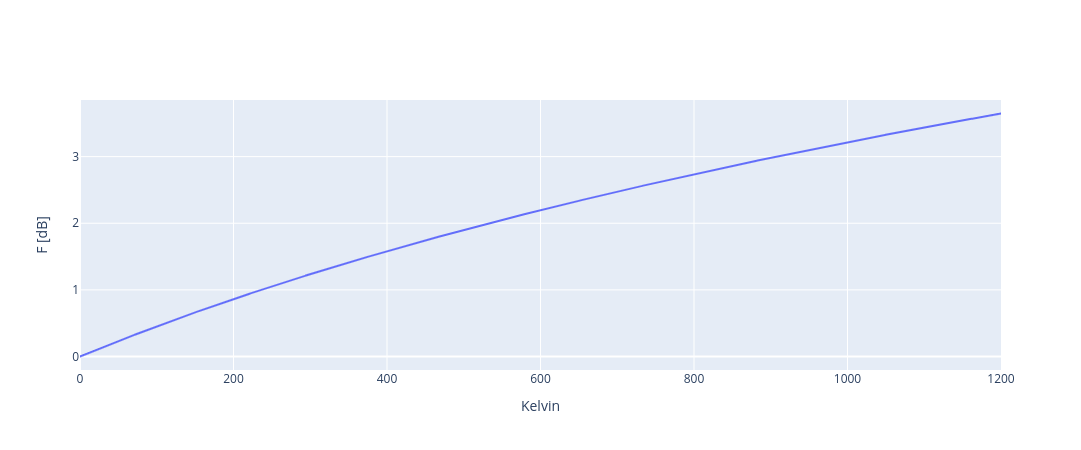
\includegraphics[width=\columnwidth]{hw5_q6.png}

\end{document}